\subsection{User Experiments}\label{subsec:userexp}

The entire Drive-LaB system has been tested through an end user experiment involving a subset of users. The experiment includes 10 drivers, who have been instructed to use the system for all their vehicular trips. To get started, all users received a two-page guide for setting up Drive-LaB on their smartphone. This guide can be seen in Appendices. The experiment ran from the 1st of May till the 3rd of June. As a motivator for using the system thoroughly, a competition was hosted, offering a prize for the user with the lowest average score percentage. The competition could be followed live through the application, allowing the drivers to monitor current results and compare them with other participants. At the end of the competition the 10 users completed 345 trips spanning 8.191 kilometers.

\begin{figure*}[!]
\centering
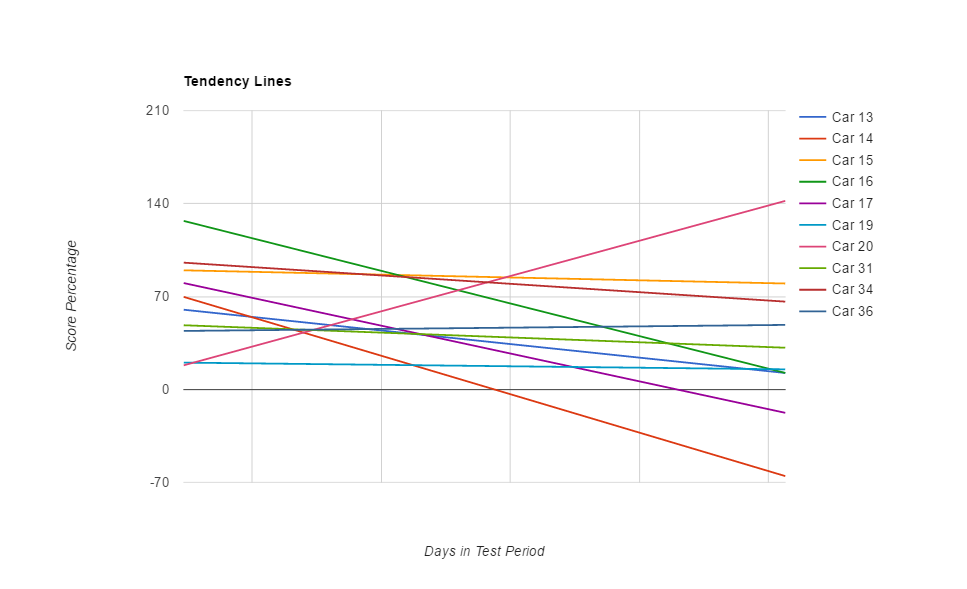
\includegraphics[width=0.80\textwidth]{Pictures/tendenslinjer}
\caption{A line chart showing the tendency lines for each individual driver}
\label{fig:tendencylines}
\end{figure*}

\begin{figure*}[!]
\centering
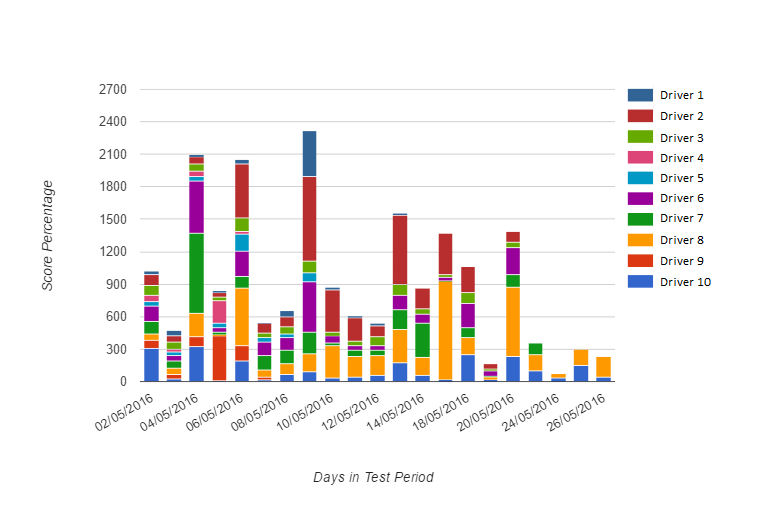
\includegraphics[width=0.80\textwidth]{Pictures/summationoftripscore}
\caption{A summation of scores based on days}
\label{fig:summationoftripscore}

\end{figure*}

There are several points to asses in this experiment, and one of them is to test the system in its entirety, in a setting true to the environment where the system will eventually be released. This test setup is as true to the real setting as possible. The frontend application was deployed on Google Play, where participants could downloaded from. Throughout the experiment, participants had access to a leaderboard with average scores for all participants. 
It would be desirable to receive user inputs on the system, to learn about perceived ease of use and possible improvements. As of the publishing of this paper, that feedback is still on its way.

One of the more interesting things to investigate through this experiment, is whether participants improve their score percentages over time. Figure \ref{fig:tendencylines} shows tendency lines for every participant throughout the experiment. It is important to notice this is merely tendency lines and not projection lines. Figure \ref{fig:tendencylines} shows a downward trend for 8 of the 10 drivers, with slope ratios between -0,284 and 3,273. It shows an upward trend for two of the drivers, with slope ratios at 0,13 and 3,54. The highest numerical slope ratios represents the drivers with the fewest amount of trips, and drivers with 0 trips later in the test period. What these results reveal, is that users of the system scores slightly better when having used the system for a period of time. This could mean that users of the system slowly improve their driving habits, dependent on the system indicating when they are actually a good driver.

Lastly, there is an interesting point to whether or not there is an incentive to keep using the system. As mentioned, the winner of the experiment received a prize at the end. As shown in Figure \ref{fig:summationoftripscore} there is a slight negative tendency in score summation, but it roughly correlates with the negative slope ratios of the tendencies in trip percentages. This means there was incentive enough to keep using the system, with the given prize. In a future insurance environment the incentive could be a cheaper insurance for the end user or engaging competitions.
 